% Provenance (never printed): old seconde/premiere S material on soil as a
% slowly renewed resource (alteration of rocks, clays, the clay--humus
% complex, soil erosion); see sources/book2/PROVENANCE.md. Rates are the
% medians of Montgomery (2007), computed in figdata/grade-10/soil_rates.py.
\chapter{El suelo, un recurso de formación lenta}\label{ch:g10:soil-formation}

Un desmonte de carretera abierto en una ladera del trópico húmedo deja ver
una pared de tierra roja de varias veces la altura de una persona. Al pie, la
roca todavía se reconoce: pálida, veteada, pero tan blanda que se desmenuza
entre los dedos sin dejar de mostrar los granos y las bandas de la roca que
fue. Hacia arriba se convierte en una arcilla moteada, después en una capa
roja y dura, y después en un suelo delgado donde están las raíces. Toda la
pared fue un día roca maciza: es la propia roca, transformada lentamente en
su sitio por el agua y el aire. El suelo, en el que crecen todas las plantas
de las tierras emergidas y los alimentos de casi toda la humanidad, es la
parte alta de una columna así. Este capítulo explica cómo la roca se
convierte en suelo, qué química hace el trabajo, cómo el clima marca su ritmo
y por qué el suelo, tan lento en formarse, puede perderse tan deprisa.

\begin{omfigure}
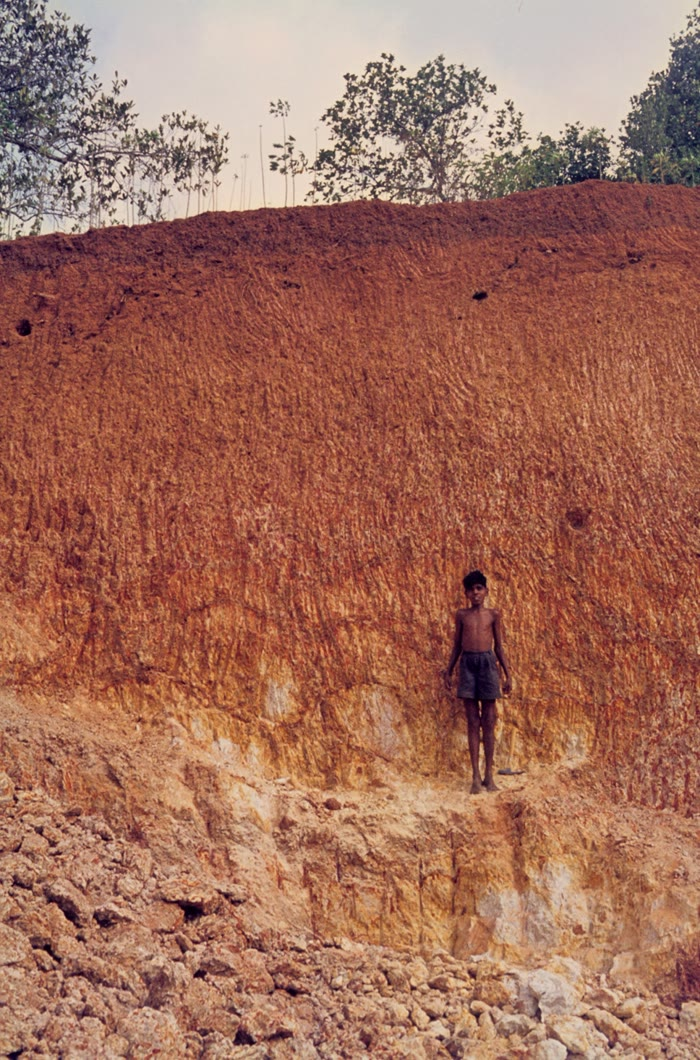
\includegraphics[height=8.5cm]{images/book2/g10-laterite-kerala.jpg}

{\small Un perfil de meteorización sobre un gneis granítico en Kerala, en el
sur de la India: abajo, una roca descompuesta y moteada; encima, una \omterm{def:g10:soil-formation:laterite}{laterita}
parda, poco endurecida, bajo un suelo delgado. El niño da la escala.
Fotografía: Werner Schellmann, 1969 (CC~BY-SA~2.5).}
\end{omfigure}

\begin{recall}
La meteorización rompe las rocas allí donde están; la erosión se lleva los
trozos; la sedimentación los deposita en otro lugar (Libro 1, año 5). Las
rocas están hechas de minerales, como el cuarzo, los feldespatos y las micas
de un granito (Libro 1, año 6). Un suelo es una capa viva de granos
minerales, humus, agua, aire y organismos; los descomponedores transforman la
materia muerta en humus; un suelo se describe por sus capas, u horizontes
(los libros de biología). En una oxidación, una sustancia pierde electrones,
a menudo al combinarse con el oxígeno (los libros de química).
\end{recall}

\section{De la roca al suelo}

La meteorización física --- la acción del hielo, el calentamiento y el
enfriamiento, las raíces --- rompe la roca en trozos sin cambiar sus
minerales. La \omterm{def:g10:soil-formation:chemical-weathering}{meteorización química} cambia los propios minerales. Juntas, a
lo largo de mucho tiempo, convierten la parte alta de la roca maciza en un
manto suelto que se engrosa hacia abajo a medida que la meteorización va
penetrando en la roca subyacente.

\begin{definition}[Roca madre; saprolita]\label{def:g10:soil-formation:weathering-profile}
La \emph{roca madre}\index{roca madre} de un suelo es la roca a partir de la
cual se formó su parte mineral. La \emph{saprolita}\index{saprolita} es una
roca descompuesta en su sitio por la meteorización: blanda y terrosa, todavía
muestra los granos y la estructura de la roca madre. Un \emph{perfil de
meteorización} es la columna completa que va de la roca sana, pasando por la
saprolita, hasta el suelo de arriba.
\end{definition}
% ledger: usgs:saprolite

La \omterm{def:g10:soil-formation:weathering-profile}{saprolita} puede ser gruesa. Bajo las colinas onduladas del flanco oriental
de los montes Apalaches, en el este de Estados Unidos, alcanza en algunos
lugares unos \qty{46}{m} (150 pies), aunque su espesor varía mucho de un
lugar a otro; el suelo es solo su parte superior.
% ledger: usgs:saprolite

\begin{omfigure}
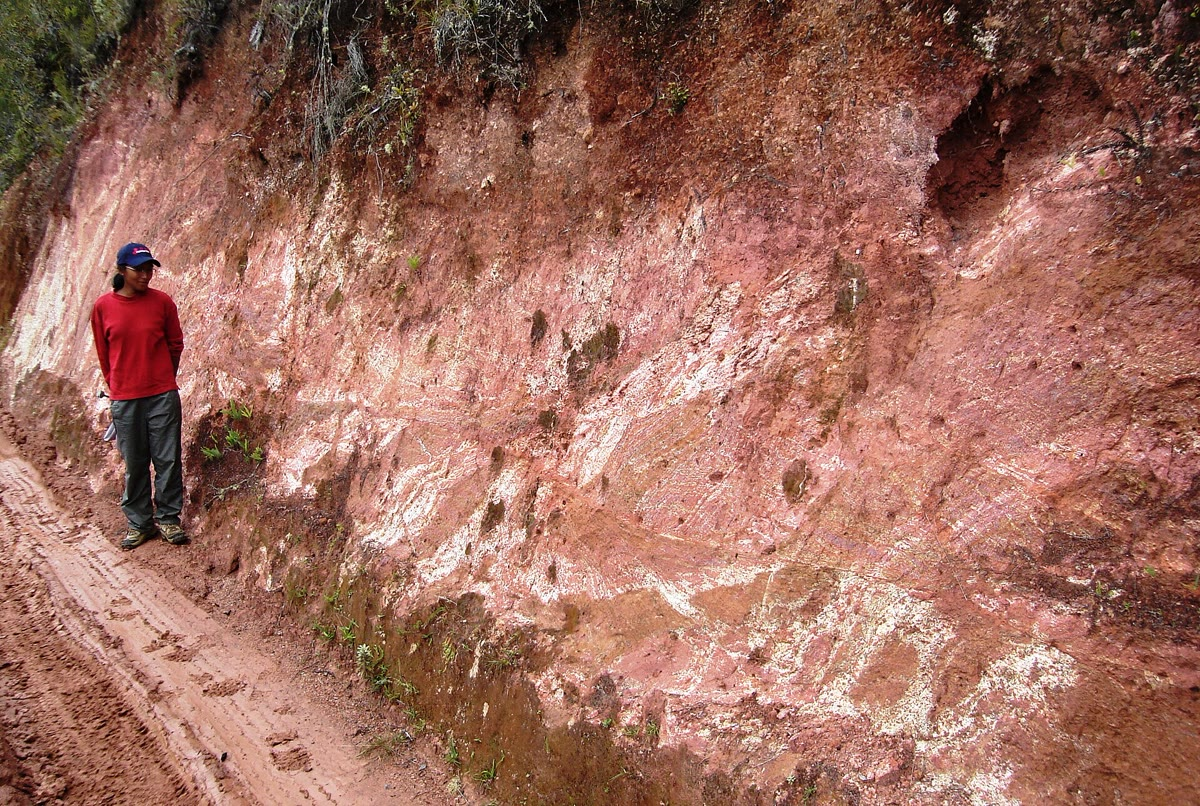
\includegraphics[width=0.8\linewidth]{images/book2/g10-saprolite-madagascar.jpg}

{\small \omterm{def:g10:soil-formation:weathering-profile}{Saprolita} en un desmonte de carretera del centro de Madagascar: el
antiguo gneis, descompuesto en su sitio, todavía muestra sus bandas como
vetas de arcilla blanca en una tierra roja. Fotografía: Diorit (CC~BY-SA~3.0).}
\end{omfigure}

\begin{omfigure}
\begin{tikzpicture}[font=\footnotesize]
  % humid tropical column
  \begin{scope}
    \fill[omThm!45!brown!60] (0,5.4) rectangle (1.8,6.0);
    \fill[omThm!70!orange!70] (0,4.2) rectangle (1.8,5.4);
    \fill[omThm!25!orange!35] (0,1.2) rectangle (1.8,4.2);
    \foreach \y in {1.5,2.1,2.7,3.3,3.9} \draw[white!80!black, thick] (0.1,\y) -- (1.7,\y+0.15);
    \fill[black!30] (0,0) rectangle (1.8,1.2);
    \foreach \x/\y in {0.3/0.3,0.9/0.7,1.4/0.2,0.5/0.9,1.2/1.0} \draw[black!55] (\x,\y) -- ++(0.2,0.08);
    \draw[black!60] (0,0) rectangle (1.8,6.0);
    \node[anchor=north, align=center] at (0.9,-0.1) {trópico\\húmedo};
  \end{scope}
  % temperate column
  \begin{scope}[xshift=3.2cm]
    \fill[omThm!45!brown!60] (0,2.2) rectangle (1.8,2.6);
    \fill[omThm!25!orange!35] (0,1.2) rectangle (1.8,2.2);
    \foreach \y in {1.5,1.9} \draw[white!80!black, thick] (0.1,\y) -- (1.7,\y+0.15);
    \fill[black!30] (0,0) rectangle (1.8,1.2);
    \foreach \x/\y in {0.3/0.3,0.9/0.7,1.4/0.2,0.5/0.9,1.2/1.0} \draw[black!55] (\x,\y) -- ++(0.2,0.08);
    \draw[black!60] (0,0) rectangle (1.8,2.6);
    \node[anchor=north, align=center] at (0.9,-0.1) {clima\\templado};
  \end{scope}
  % labels
  \draw[black!50] (5.3,5.7) -- (2.0,5.7); \node[anchor=west] at (5.4,5.7) {suelo};
  \draw[black!50] (5.3,4.8) -- (2.0,4.8); \node[anchor=west, align=left] at (5.4,4.8) {laterita: roja, rica en óxidos\\de hierro y de aluminio};
  \draw[black!50] (5.3,3.4) -- (2.0,3.4); \node[anchor=west, align=left] at (5.4,3.4) {saprolita: roca descompuesta\\en su sitio, con su estructura};
  \draw[black!50] (5.3,0.6) -- (5.0,0.6); \node[anchor=west] at (5.4,0.6) {roca madre sana};
\end{tikzpicture}

{\small Dos perfiles de meteorización sobre la misma roca (esquema, sin
escala): bajo un clima cálido y húmedo el perfil es mucho más grueso y su
parte alta es una \omterm{def:g10:soil-formation:laterite}{laterita}; bajo un clima templado, una \omterm{def:g10:soil-formation:weathering-profile}{saprolita} más
delgada sostiene el suelo.}
\end{omfigure}

\section{La meteorización química}

\begin{definition}[Meteorización química]\label{def:g10:soil-formation:chemical-weathering}
La \emph{meteorización química}\index{meteorizacion quimica@meteorización química}
es la transformación de los minerales de una roca por reacciones con el agua
y con los gases que lleva, el dióxido de carbono y el oxígeno: algunos
minerales se disuelven, otros se convierten en minerales nuevos, estables en
la superficie de la Tierra.
\end{definition}

El agua de lluvia disuelve un poco de dióxido de carbono del aire, y mucho
más al infiltrarse en el suelo, donde las raíces y los descomponedores lo
expulsan al respirar. Parte del gas disuelto forma ácido carbónico, que
libera iones hidrógeno:
\begin{center}
\ce{CO2 + H2O -> H+ + HCO3-}
\end{center}
Estos iones hidrógeno atacan los minerales.

\begin{definition}[Hidrólisis]\label{def:g10:soil-formation:hydrolysis}
La \emph{hidrólisis}\index{hidrolisis@hidrólisis} es la \omterm{def:g10:soil-formation:chemical-weathering}{meteorización química}
de un mineral silicatado por el agua y sus iones hidrógeno: los iones
hidrógeno ocupan el lugar de los iones metálicos del mineral, que pasan a la
disolución, y el resto del mineral se reorganiza en un \omterm{def:g10:soil-formation:clay}{mineral de la arcilla}.
\end{definition}

\begin{proposition}[Hidrólisis de un feldespato]\label{prop:g10:soil-formation:hydrolysis}
La \omterm{def:g10:soil-formation:hydrolysis}{hidrólisis} transforma el feldespato potásico ortosa, \ce{KAlSi3O8}, en el
\omterm{def:g10:soil-formation:clay}{mineral de la arcilla} caolinita, \ce{Al2Si2O5(OH)4}; el agua se lleva iones
potasio y sílice disuelta, \ce{H4SiO4}:
\begin{center}
\ce{2 KAlSi3O8 + 2 H+ + 9 H2O -> Al2Si2O5(OH)4 + 2 K+ + 4 H4SiO4}
\end{center}
\end{proposition}
% ledger: webmineral:formulas

\begin{proof}[Comprobación]
Cuenta cada elemento en los dos miembros. Potasio: 2 y 2. Aluminio: 2 y 2.
Silicio: 6 y $2 + 4 = 6$. Oxígeno: $16 + 9 = 25$ y $9 + 16 = 25$.
Hidrógeno: $2 + 18 = 20$ y $4 + 16 = 20$. Carga: $+2$ y $+2$.
\end{proof}

\begin{proposition}[Disolución de la calcita]\label{prop:g10:soil-formation:calcite}
La calcita, \ce{CaCO3}, el mineral de la caliza, se disuelve por completo en
un agua que lleva dióxido de carbono; no queda nada sólido:
\begin{center}
\ce{CaCO3 + CO2 + H2O -> Ca^2+ + 2 HCO3-}
\end{center}
\end{proposition}
% ledger: webmineral:formulas

El hierro sufre un tercer tipo de ataque. En los minerales oscuros de una
roca, como la mica negra de un granito, el hierro está en la forma reducida
\ce{Fe^2+}. El oxígeno que lleva el agua lo oxida, y el hierro(III) se queda
en forma de óxidos insolubles: la goethita, de color pardo amarillento,
\ce{FeO(OH)}, y la hematites, roja, \ce{Fe2O3}. Para la goethita:
\begin{center}
\ce{4 Fe^2+ + O2 + 6 H2O -> 4 FeO(OH) + 8 H+}
\end{center}
Estos óxidos tiñen de amarillo, pardo y rojo las rocas meteorizadas y los
suelos.
% ledger: webmineral:formulas

No todos los minerales se meteorizan al mismo ritmo. En un granito que se
meteoriza, la mica negra se oxida y los feldespatos se convierten en arcilla,
pero los granos de cuarzo, casi insolubles, salen intactos: acaban siendo
arena.

\begin{example}[La meteorización de un granito]\label{ex:g10:soil-formation:granite}
% ledger: webmineral:formulas (masses computed in figdata/grade-10/soil_rates.py)
Un kilogramo de ortosa contiene $1000/278.33 \approx \qty{3.59}{mol}$ de
\ce{KAlSi3O8}. Según la ecuación, dos moles de ortosa dan un mol de
caolinita: $3.59/2 \approx \qty{1.80}{mol}$, es decir, $1.80 \times 258.16
\approx \qty{464}{g}$ de arcilla. El potasio, el $14.05~\%$ de la masa de la
ortosa, \qty{140.5}{g}, y $2 \times 3.59 = \qty{7.19}{mol}$ de sílice
se van en disolución. De un granito de cuarzo, feldespatos y micas, la
meteorización deja arena (el cuarzo), arcilla (de los feldespatos y las
micas) y óxidos de hierro, y envía a los ríos potasio, sodio, calcio y sílice.
\end{example}

\section{Las arcillas y el humus}

\begin{definition}[Mineral de la arcilla]\label{def:g10:soil-formation:clay}
Un \emph{mineral de la arcilla}\index{mineral de la arcilla} es un silicato
formado por láminas finas de átomos apiladas unas sobre otras, nacido de la
meteorización, que se presenta en escamas mucho más pequeñas que los granos
de arena. La caolinita es uno de ellos.
\end{definition}
% ledger: webmineral:formulas

Las superficies de las escamas de arcilla llevan cargas eléctricas negativas.
Retienen iones positivos --- potasio \ce{K+}, calcio \ce{Ca^2+}, magnesio
\ce{Mg^2+}, amonio \ce{NH4+} --- que de otro modo la lluvia arrastraría.
El humus hace lo mismo. Unidos, la arcilla y el humus forman el
\emph{complejo arcilloso-húmico}, la reserva de nutrientes minerales del
suelo: una raíz libera iones hidrógeno y toma a cambio el potasio o el calcio
retenidos en las escamas.

\begin{omfigure}
\begin{tikzpicture}[font=\footnotesize, >={Stealth[length=2mm]}]
  \foreach \y in {0,0.7,1.4} {
    \fill[omExo!35, draw=black!60] (0,\y) rectangle (7.2,\y+0.3);
    \foreach \x in {0.3,0.9,...,7.0} \node[font=\tiny, black!70] at (\x,\y+0.15) {$-$};
  }
  \foreach \x/\ion in {0.7/K^+, 1.9/Ca^{2+}, 3.1/K^+, 4.3/Mg^{2+}, 5.5/NH_4^+, 6.7/K^+} {
    \fill[omThm!20, draw=omThm!80!black] (\x,2.1) circle (0.4);
    \node[font=\scriptsize] at (\x,2.1) {$\mathrm{\ion}$};
  }
  \foreach \x in {1.3, 3.7, 6.1} \fill[omThm!20, draw=omThm!80!black] (\x,0.5) circle (0.17);
  \foreach \x in {2.5, 4.9} \fill[omThm!20, draw=omThm!80!black] (\x,1.2) circle (0.17);
  \node[anchor=north] at (3.6,-0.1) {láminas de arcilla con carga negativa e iones positivos entre ellas};
  \node[anchor=south] at (3.1,2.5) {iones positivos retenidos en las superficies};
  % root and exchange
  \draw[line width=2.2pt, brown!60!black] (9.6,3.4) .. controls (9.3,2.6) and (8.9,2.2) .. (8.1,2.0);
  \node[anchor=east] at (9.25,3.3) {raíz};
  \draw[->, omDef!80!black, thick] (8.0,2.2) .. controls (7.6,2.6) and (7.2,2.6) .. (6.95,2.3);
  \node[anchor=south, omDef!80!black] at (7.5,2.55) {\ce{H+} cedido};
  \draw[->, omThm!80!black, thick] (6.95,1.8) .. controls (7.3,1.5) and (7.7,1.6) .. (8.0,1.85);
  \node[anchor=north, omThm!80!black] at (7.8,1.55) {\ce{K+} tomado};
\end{tikzpicture}

{\small El complejo arcilloso-húmico (esquema): las láminas de arcilla, con
carga negativa, retienen iones positivos en sus superficies y entre ellas;
una raíz intercambia iones hidrógeno por estos nutrientes.}
\end{omfigure}

\section{Los suelos y el clima}

La \omterm{def:g10:soil-formation:chemical-weathering}{meteorización química} necesita agua y, como la mayoría de las reacciones,
va más deprisa cuando hace calor. Donde el clima es a la vez cálido y húmedo,
la roca se descompone más hondo y más a fondo: los feldespatos se convierten
por completo en arcilla, incluso buena parte de la sílice se va, y lo que
queda es rico en los elementos menos solubles, el hierro y el aluminio.

\begin{definition}[Laterita]\label{def:g10:soil-formation:laterite}
Una \emph{laterita}\index{laterita} es un material profundamente meteorizado
de los climas cálidos y húmedos, rojo o pardo, formado sobre todo por óxidos
de hierro y de aluminio y por caolinita, del que se ha eliminado casi todo lo
soluble.
\end{definition}

Bajo los climas fríos, helados buena parte del año, y bajo los climas secos,
donde el agua escasea, la \omterm{def:g10:soil-formation:chemical-weathering}{meteorización química} es lenta: los suelos son
delgados y la roca está muy cerca, justo debajo. Entre los polos y el
ecuador, la profundidad de la meteorización es máxima bajo las selvas
tropicales húmedas y mínima en los desiertos y en las regiones polares.

\begin{omfigure}
\begin{tikzpicture}[font=\footnotesize]
  \fill[black!25] (0,-0.2) -- (0,-0.5) .. controls (1.5,-0.6) and (2.5,-1.4) .. (3.4,-1.2)
     .. controls (4.2,-1.0) and (4.6,-0.55) .. (5.2,-0.5) .. controls (6.0,-0.5) and (6.6,-1.6) .. (7.6,-3.0)
     .. controls (8.2,-3.6) and (9.0,-3.6) .. (10,-3.4) -- (10,-3.8) -- (0,-3.8) -- cycle;
  \fill[omThm!25!orange!35] (0,0) -- (10,0) -- (10,-3.4) .. controls (9.0,-3.6) and (8.2,-3.6) .. (7.6,-3.0)
     .. controls (6.6,-1.6) and (6.0,-0.5) .. (5.2,-0.5) .. controls (4.6,-0.55) and (4.2,-1.0) .. (3.4,-1.2)
     .. controls (2.5,-1.4) and (1.5,-0.6) .. (0,-0.5) -- cycle;
  \draw[black!60] (0,0) -- (10,0);
  \node[anchor=south] at (0.6,0.05) {polar};
  \node[anchor=south] at (3.2,0.05) {templado};
  \node[anchor=south] at (5.3,0.05) {desierto};
  \node[anchor=south] at (6.8,0.05) {sabana};
  \node[anchor=south] at (9.0,0.05) {selva tropical};
  \node[anchor=north] at (0.4,-3.85) {polo};
  \node[anchor=north] at (9.6,-3.85) {ecuador};
  \node[black!70] at (2.0,-2.6) {roca sana};
  \node[black!80] at (8.35,-1.0) {roca meteorizada y suelo};
\end{tikzpicture}

{\small La profundidad de la meteorización desde un polo hasta el ecuador
(esquema, profundidades sin escala): pequeña bajo los climas polares y
desérticos, moderada bajo los climas templados, máxima bajo las selvas
tropicales húmedas.}
\end{omfigure}

\section{Lento en formarse, rápido en perderse}

¿A qué velocidad se forma el suelo? La producción de suelo, el ritmo al que
la meteorización convierte la roca en suelo en la base del perfil, se ha
medido en muchos lugares del mundo, igual que el ritmo al que el suelo se
erosiona en la superficie. Una recopilación de estas medidas da los ritmos
típicos (medianos) que siguen, cada uno expresado como un espesor de suelo
por año.
% ledger: montgomery:rates

\begin{omfigure}
\begin{tikzpicture}
\begin{axis}[omrecord, width=0.82\linewidth, height=5.6cm, ymode=log, log origin=infty, ymin=0.005,
  ymax=5, ybar, bar width=16pt, xtick={0,1,2,3,4}, xmin=-0.6, xmax=4.6,
  xticklabels={{producción\\de suelo}, {erosión con\\vegetación natural}, {erosión\\geológica}, {agricultura de\\conservación}, {arado\\convencional}},
  xticklabel style={align=center, font=\scriptsize},
  ylabel={ritmo (\unit{mm} por año)}, tick label style={font=\small}, label style={font=\small},
  nodes near coords, nodes near coords style={font=\scriptsize}, point meta=explicit symbolic]
\addplot[fill=omDef!45, draw=omDef!80!black] table[x=idx, y=rate_mm_yr, meta=rate_mm_yr] {figdata/out/grade-10-soil_rates-rates.dat};
\end{axis}
\end{tikzpicture}

{\small Ritmos medianos de producción de suelo y de erosión según una
recopilación mundial de medidas, en milímetros de suelo por año (escala
logarítmica: cada escalón es diez veces el de abajo). Datos: Montgomery
(2007), \emph{Proceedings of the National Academy of Sciences}.}
\end{omfigure}
% ledger: montgomery:rates

Bajo la vegetación natural, el suelo se erosiona más o menos tan deprisa como
se forma, unos \qty{0.02}{mm} al año: un centímetro en unos seis siglos. Con
el arado convencional, que deja el suelo desnudo entre cultivos, el ritmo
mediano de erosión es de \qty{1.5}{mm} al año, noventa veces el ritmo de
producción de suelo. Con la agricultura de conservación, que remueve menos el
suelo y lo mantiene cubierto, la mediana baja a \qty{0.08}{mm} al año, mucho
más cerca del ritmo de producción.
% ledger: montgomery:rates (ratios computed in figdata/grade-10/soil_rates.py)

\begin{method}[Comparar un ritmo de formación con un ritmo de erosión]\label{met:g10:soil-formation:rates}
\begin{enumerate}
  \item Expresa los dos ritmos en la misma unidad (milímetros por año).
  \item La pérdida neta es el ritmo de erosión $E$ menos el ritmo de
        producción $P$.
  \item Un suelo de espesor $S$ se pierde en $T = S/(E - P)$ años; si
        $E \le P$, el suelo no se está perdiendo.
  \item Formar un espesor $S$ partiendo de cero lleva $S/P$ años.
\end{enumerate}
\end{method}
% ledger: montgomery:lifetime

Con estos ritmos, un metro de suelo tarda unos $1000/0.017 \approx 59\,000$
años en formarse, y con el arado convencional puede perderse en unos
$1000/(1.537 - 0.017) \approx 660$ años. A la escala del tiempo humano, el
suelo es un recurso que no se renueva.
% ledger: montgomery:rates, montgomery:lifetime

\begin{omfigure}
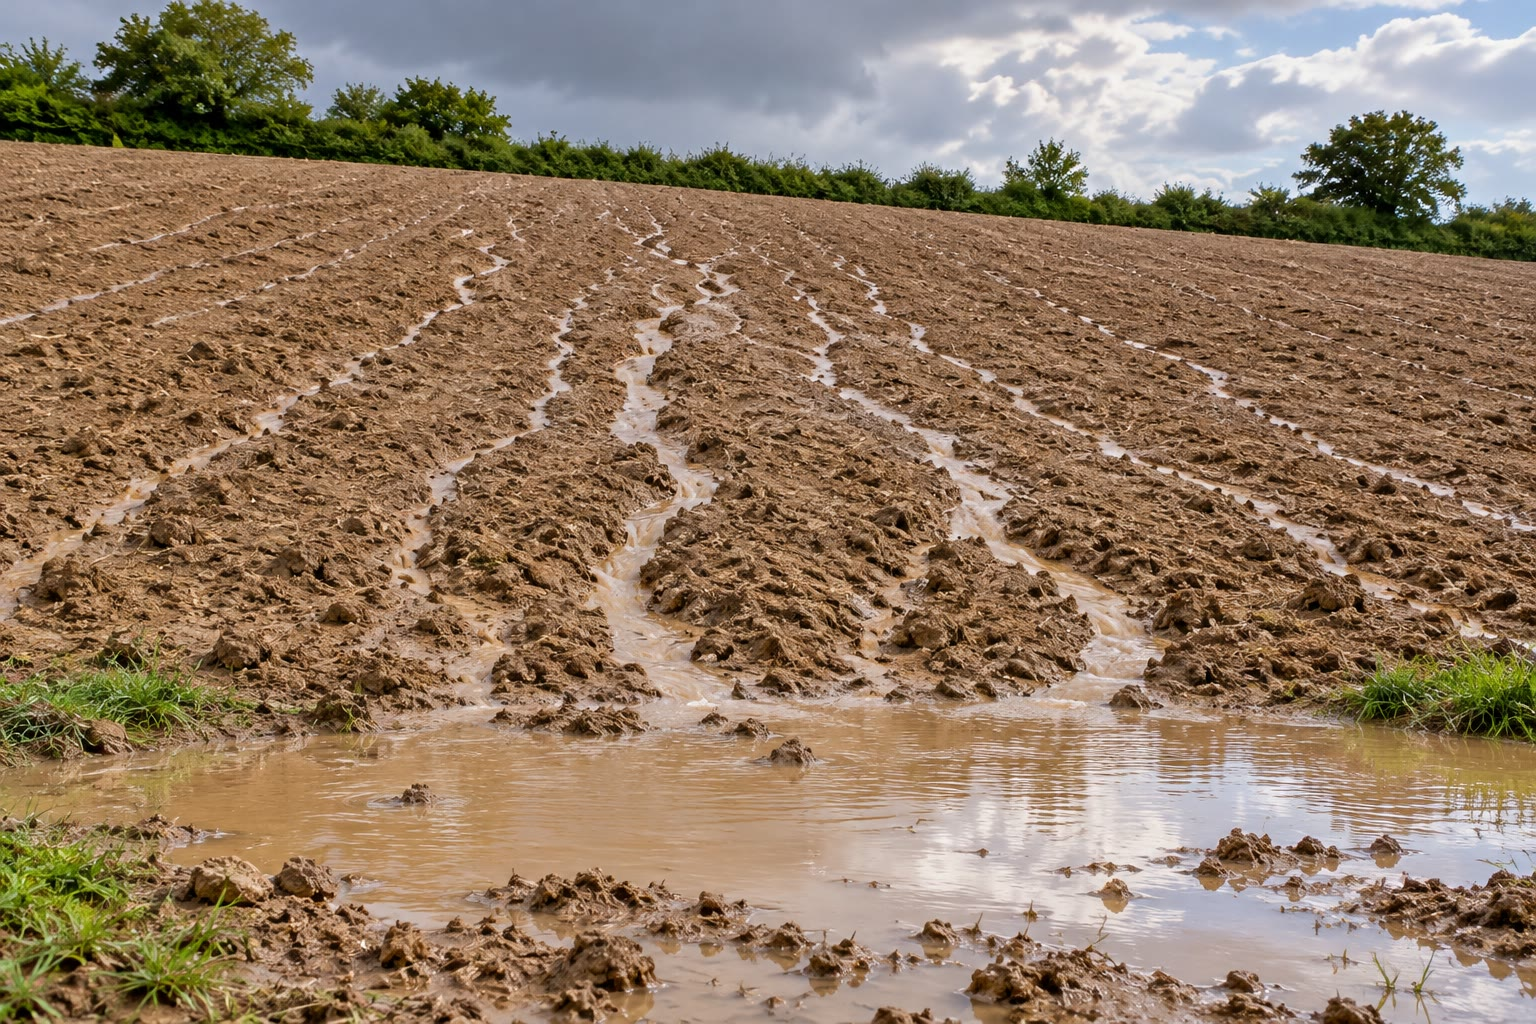
\includegraphics[width=0.72\linewidth]{images/book2/ai/g10-ploughed-rills.jpg}

{\small Un campo arado después de una fuerte tormenta: la escorrentía ha
excavado pequeños canales, o regueros, pendiente abajo y ha arrastrado el
suelo hasta un charco de barro al pie.}
\end{omfigure}

\section{Ejercicios}

\begin{exercise}[$\star$]\label{exo:g10:soil-formation:1}
Define la \omterm{def:g10:soil-formation:chemical-weathering}{meteorización química} y la \omterm{def:g10:soil-formation:hydrolysis}{hidrólisis}.
\end{exercise}

\begin{exercise}[$\star$]\label{exo:g10:soil-formation:2}
¿Qué es la \omterm{def:g10:soil-formation:weathering-profile}{saprolita}? ¿Cómo distinguirías una \omterm{def:g10:soil-formation:weathering-profile}{saprolita} de un suelo formado
sobre arena traída por un río?
\end{exercise}

\begin{exercise}[$\star$]\label{exo:g10:soil-formation:3}
Nombra los productos de la meteorización de un granito: ¿en qué se convierte
cada uno de sus tres minerales principales?
\end{exercise}

\begin{exercise}[$\star$]\label{exo:g10:soil-formation:4}
¿Por qué las rocas meteorizadas y los suelos tropicales son tan a menudo
rojos, amarillos o pardos?
\end{exercise}

\begin{exercise}[$\star$]\label{exo:g10:soil-formation:5}
Con el diagrama de barras, da el ritmo mediano de producción de suelo y el
ritmo mediano de erosión con el arado convencional. ¿Cuántas veces mayor es
el segundo?
\end{exercise}

\begin{exercise}[$\star\star$]\label{exo:g10:soil-formation:6}
Comprueba que la ecuación de la disolución de la calcita está ajustada, para
cada elemento y para la carga.
\end{exercise}

\begin{exercise}[$\star\star$]\label{exo:g10:soil-formation:7}
La caliza se disuelve por completo; el granito deja arena y arcilla. Explica
la diferencia con ayuda de las dos reacciones del capítulo.
\end{exercise}

\begin{exercise}[$\star\star$]\label{exo:g10:soil-formation:8}
Explica cómo el complejo arcilloso-húmico retiene el potasio en un suelo que
la lluvia atraviesa, y cómo lo toma una raíz.
\end{exercise}

\begin{exercise}[$\star\star$]\label{exo:g10:soil-formation:9}
Da dos razones por las que las \omterm{def:g10:soil-formation:laterite}{lateritas} se forman bajo climas cálidos y
húmedos y no bajo climas fríos o secos.
\end{exercise}

\begin{exercise}[$\star\star$]\label{exo:g10:soil-formation:10}
El ritmo mediano de producción de suelo es de \qty{0.017}{mm} al año. ¿Cuánto
tiempo hace falta para formar \qty{1}{cm}, \qty{30}{cm} y \qty{1}{m} de suelo?
\end{exercise}

\begin{exercise}[$\star\star$]\label{exo:g10:soil-formation:11}
Los ritmos de erosión se dan a menudo como una masa de suelo por hectárea y
por año. Con una densidad del suelo de \qty{1200}{kg/m^3}, ¿qué masa
representa una pérdida de \qty{1.5}{mm} al año en una hectárea
(\qty{10000}{m^2})?
\end{exercise}

\begin{exercise}[$\star\star\star$]\label{exo:g10:soil-formation:12}
Bajo las colinas de una región templada se ha formado una \omterm{def:g10:soil-formation:weathering-profile}{saprolita} de
\qty{46}{m} de espesor. Si la meteorización avanzara en la roca a
\qty{0.017}{mm} al año, ¿cuánto tiempo habría hecho falta? ¿Qué sugiere la
respuesta sobre la edad de un paisaje así?
\end{exercise}

\begin{exercise}[$\star\star\star$]\label{exo:g10:soil-formation:13}
Escribe la ecuación de la oxidación del \ce{Fe^2+} en goethita que da el
capítulo y compruébala. Después escribe y ajusta la oxidación del \ce{Fe^2+}
en hematites, \ce{Fe2O3}, por el oxígeno y el agua, con liberación de \ce{H+}.
\end{exercise}

\begin{exercise}[$\star\star\star$]\label{exo:g10:soil-formation:14}
Con la agricultura de conservación, el ritmo mediano de erosión es de
\qty{0.082}{mm} al año. Con una producción de suelo de \qty{0.017}{mm} al
año, ¿cuánto tiempo se tarda en perder \qty{30}{cm} de suelo? Compáralo con
el arado convencional.
\end{exercise}

\begin{exercise}[$\star\star\star$]\label{exo:g10:soil-formation:15}
Un granito contiene un \qty{30}{\percent} de ortosa en masa. ¿Qué masa de
caolinita se forma cuando toda la ortosa de una tonelada de este granito se
ha meteorizado, y qué masa de potasio se libera?
\end{exercise}

\section{Problema: la vida de un suelo}

\begin{problem}[{Problema de fin de semana --- de la roca al campo y de vuelta al río}]
\label{pb:g10:soil-formation:1}
% ledger: montgomery:rates, montgomery:lifetime, webmineral:formulas (values computed in figdata/grade-10/soil_rates.py)

\begin{center}
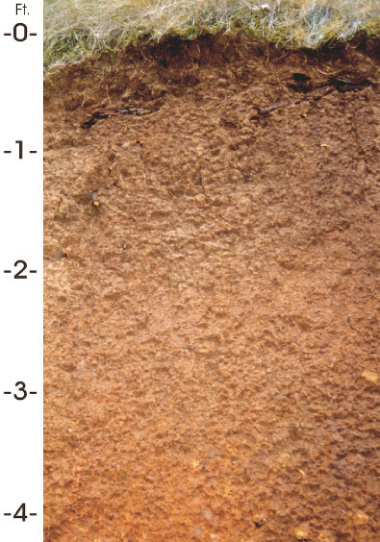
\includegraphics[height=6cm]{images/book2/g10-nrcs-jory-soil.jpg}

{\small Un perfil de suelo, con una escala en pies a la izquierda
(\num{1}~pie = \qty{0.3048}{m}). Fotografía: USDA Natural Resources
Conservation Service (dominio público).}
\end{center}

\medskip
\noindent\textbf{Parte I --- Un perfil.}
\begin{enumerate}
  \item La escala llega a 4 pies cerca del borde inferior de la imagen. ¿Qué
        profundidad es esa, en metros?
  \item La capa oscura de arriba llega a cerca de medio pie. ¿Qué espesor
        tiene, en centímetros?
  \item ¿Qué da a esta capa superior su color oscuro?
  \item Más abajo, el suelo es de color pardo rojizo. ¿Qué minerales le dan
        este color, y cómo se formaron?
  \item ¿Se ve la \omterm{def:g10:soil-formation:weathering-profile}{roca madre} en la fotografía? ¿Qué esperarías encontrar por
        debajo del borde inferior de la imagen?
\end{enumerate}

\medskip
\noindent\textbf{Parte II --- La química de un granito que se meteoriza.}
\begin{enumerate}[resume]
  \item Escribe la ecuación de la \omterm{def:g10:soil-formation:hydrolysis}{hidrólisis} de la ortosa.
  \item ¿Cuántos moles de ortosa hay en \qty{1}{kg}
        (\qty{278.33}{g/mol})?
  \item ¿Qué masa de caolinita (\qty{258.16}{g/mol}) dan?
  \item ¿Qué se va con el agua, y adónde va?
  \item ¿Qué le ocurre al cuarzo del granito?
\end{enumerate}

\medskip
\noindent\textbf{Parte III --- Formación frente a erosión.}
\begin{enumerate}[resume]
  \item El suelo se forma a \qty{0.017}{mm} al año. ¿Cuánto tiempo tarda en
        formarse el perfil de la Parte I?
  \item Con el arado convencional, el suelo se erosiona a \qty{1.537}{mm} al
        año. ¿Cuál es la pérdida neta cada año?
  \item ¿Cuánto duraría el perfil de la Parte I?
  \item Compara los dos tiempos de las preguntas 11 y 13.
  \item Bajo la vegetación natural, la erosión es de \qty{0.013}{mm} al año.
        ¿Se está perdiendo el suelo?
\end{enumerate}

\medskip
\noindent\textbf{Parte IV --- La vida de un suelo.}
\begin{enumerate}[resume]
  \item Escribe el tiempo $T$ que se tarda en perder un espesor $S$ de suelo
        en función de $S$, del ritmo de erosión $E$ y del ritmo de producción
        $P$.
  \item Calcula $T$ para $S = \qty{30}{cm}$ con el arado convencional.
  \item Calcula $T$ para $S = \qty{30}{cm}$ con la agricultura de
        conservación (\qty{0.082}{mm} al año).
  \item ¿Por qué se puede decir que un suelo es un recurso que no se renueva
        a la escala del tiempo humano?
  \item ¿Cuánto tiempo se tarda en perder un metro de suelo con el arado
        convencional?
\end{enumerate}
\end{problem}
